\documentclass{beamer}

\usepackage[czech]{babel}
\usepackage[utf8]{inputenc}
\usepackage{multicol}
\usepackage[backend=bibtex, style=iso-numeric, alldates=iso]{biblatex}

\usetheme{Madrid}
\usecolortheme{default}% - nic / default == modrá

\title{Webová služba pro sběr a vizualizaci předpovědí počasí}
\subtitle{Web Service for Collection and Visualization of Weather Forecasts}
\author{Jan Jedlička JED0050}
\institute{VŠB-TUO}
\date{2021}

\addbibresource{citace.bib}

\begin{document}
	
	\frame{\titlepage}
	
	\begin{frame}
		\frametitle{Úvod}
		
		\begin{itemize}
			\item Aplikace agregující data z různých datových zdrojů
			\item Webová služba poskytující agregovaná data
			\item Aplikace zobrazující data z webové služby
		\end{itemize}
		
	\end{frame}

	\begin{frame}
		\frametitle{Řešení}
		
		\begin{itemize}
			\item Knihovny jednotlivých datových zdrojů
			\item Knihovna pro správu různých datových zdrojů
			\item ASP.NET aplikace využívající knihovnu agregace dat
			\item Windows Forms aplikace zobrazující data z webu
		\end{itemize}
		
		\begin{figure}
			
			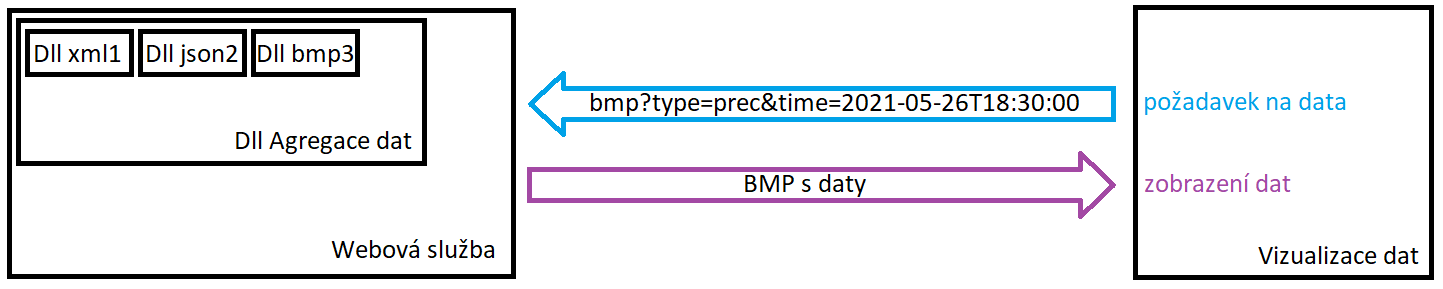
\includegraphics[scale=0.323]{figures/schema prace.png}

		\end{figure}
		
	\end{frame}

	\begin{frame}
		\frametitle{Datové zdroje}
		
		\begin{itemize}
			\item XML
			\begin{itemize}
				\item Yr.no
			\end{itemize}
			\item JSON
			\begin{itemize}
				\item OpenWeather
				\item WeatherUnlocked
			\end{itemize}
			\item BMP
			\begin{itemize}
				\item Medard
				\item Radar.bourky
			\end{itemize}
		\end{itemize}
	\end{frame}

	\begin{frame}
		\frametitle{Porovnání datových zdrojů}
		
		\begin{tabular} {l r c c c c c c c}
			
			Zkratka & Typ & Dny & Hodin rozdíl & Stažení/min & Plocha & Prvek \\
			\hline
			Yrno & XML & 9 & 1 a 6 & & svět & s,v,t1,t2 \\ 
			Owm & JSON & 5 & 3 & 60 & svět & s,v,t1,t2 \\ 
			Weun & JSON & 5 & 3 & 75 & svět & s,v,t1,t2 \\ 
			Mdrd & BMP & 5 & 1 &  & Evropa & s,t1 \\ 
			Rb & BMP & -3 & 0.16 (10 min)& & ČR & s \\ 
			\multicolumn{7}{r}{\footnotesize *s = srážky, v = vlhkost, t1 = teplota, t2 = tlak}\\
		\end{tabular}
	\end{frame}

	\begin{frame}
		\frametitle{Agregace dat - Triangulace}
		
		\begin{figure}
			
			
\includegraphics[scale=0.5]{figures/bmp_body.png}
			\caption{Množina bodů s předpověďmi}
			
		\end{figure}
	
	\end{frame}

	\begin{frame}
		\frametitle{Agregace dat - Triangulace}
		
		\begin{figure}
			
			
\includegraphics[scale=0.5]{figures/bmp_sit.png}
			\caption{Síť trojúhelníků}
			
		\end{figure}
		
	\end{frame}
	
	\begin{frame}
		\frametitle{Agregace dat - Interpolace}
		
		\begin{displaymath}
			Value_v = \frac{W_{v1}Value_{v1} + W_{v2}Value_{v2} + W_{v3}Value_{v3}}{W_{v1} + W_{v2} + W_{v3}}
		\end{displaymath}
		
		\begin{figure}
			
			
\includegraphics[scale=0.25]{figures/interpolace_trojuhelnik.jpg}
			\caption{Obsah trojúhelník dopočítaný interpolací \cite{coltrian}}
			
		\end{figure}
		
	\end{frame}
	
	\begin{frame}
		\frametitle{Agregace dat - Interpolace}
		
		\begin{figure}
			
			
\includegraphics[scale=0.5]{figures/bmp_vybarvena.png}
			\caption{Kompletní bitmapa \textbf{temp-2021-04-25-12}}
			
		\end{figure}
		
	\end{frame}

	\begin{frame}
		\frametitle{Agregace dat - Škála}
		
		\begin{itemize}
			\item Převod barev na číslo a naopak
			\item Šířka odpovídá počtu hodnot
			\item Známe hodnotu 1. pixelu a rozdíl mezi pixely
		\end{itemize}
		
		\begin{figure}
			
			
\includegraphics[scale=3]{figures/scale_temp.png}
			\caption{Škála pro teplotu}
			
		\end{figure}
		
	\end{frame}

	\begin{frame}
		\frametitle{Agregace dat - Přístup k datům}
		
		\begin{itemize}
			\item TYP-ROK-MĚSÍC-DEN-HODINA (-MINUTA)
			\item \textbf{temp-2021-04-25-12}, \textbf{prec-2023-11-23-6-30}
		\end{itemize}
		
	\end{frame}

	\begin{frame}
		\frametitle{Distribuce dat - Bitmap předpověď}
		
		\begin{itemize}			
			\item bmp?type=\textbf{prec}\&time=\textbf{2021-04-24T18:30:00}\&loaders=\textbf{owm,yrno}
			\item prec-2021-04-24-18
		\end{itemize}
		
		\begin{figure}
			
			
\includegraphics[scale=0.35]{figures/bmp_prec.PNG}
			\caption{Bitmapa s daty o srážkách}
			
		\end{figure}
		
	\end{frame}
	
	\begin{frame}[fragile]
		\frametitle{Distribuce dat - XML předpověď}
		
		\begin{itemize}
			\item \textbf{xml}?lon=\textbf{18.262524}\&lat=\textbf{49.820923}
			\&time=\textbf{2021-04-24T14:00:00}\&loaders=\textbf{mdrd,owm}
		\end{itemize}
		
		\begin{exampleblock}{Ukázka XML předpovědi}
			\begin{verbatim}
				<Coord>
				  <Lon>18.262524</Lon>
				  <Lat>49.820923</Lat>
				</Coord>
				<Forecasts>
				  <Forecast>
				    <DateTime Value="2021-04-24T14:00:00" Format="ISO 8601"/>
				    <Temperature Value="9.75" Unit="°C" />
				    <Precipitation Value="0.42" Unit="mm" />
				    <Humidity Value="57.3333" Unit="%" />
				    <Pressure Value="1022.6667" Unit="hPa" />
				  </Forecast>
				</Forecasts>
			\end{verbatim}
		\end{exampleblock}
	\end{frame}
	
	\begin{frame}[fragile]
		\frametitle{Distribuce dat - JSON předpověď}
			
			\begin{itemize}
				\item \textbf{json}?lon=\textbf{18.262524}\&lat=\textbf{49.820923}
				\&time=\textbf{2021-04-29T16:00:00}\&loaders=\textbf{weun,yrno}
			\end{itemize}
			
			\begin{exampleblock}{Ukázka JSON předpovědi}
				\begin{verbatim}
					{
					    "DataSources":["WeatherUnlocked","Yr.no"],
					    "Forecasts":
					      [{
					        "Time":"2021-04-29T16:00:00",
					        "Temperature":15.0,
					        "Precipitation":0.0,
					        "Humidity":66.0,
					        "Pressure":1007.5
				       }],
					    "Coord":{"Lon":18.262524,"Lat":49.820923}
					}
				\end{verbatim}
			\end{exampleblock}
	\end{frame}

	\begin{frame}
		\frametitle{Vizualizace dat - Počasí v bodě}
		
		\begin{itemize}
			\item Zadání prvku počasí, datových zdrojů, času a bodu (kliknutí/název)
		\end{itemize}
	
		\begin{figure}
			
			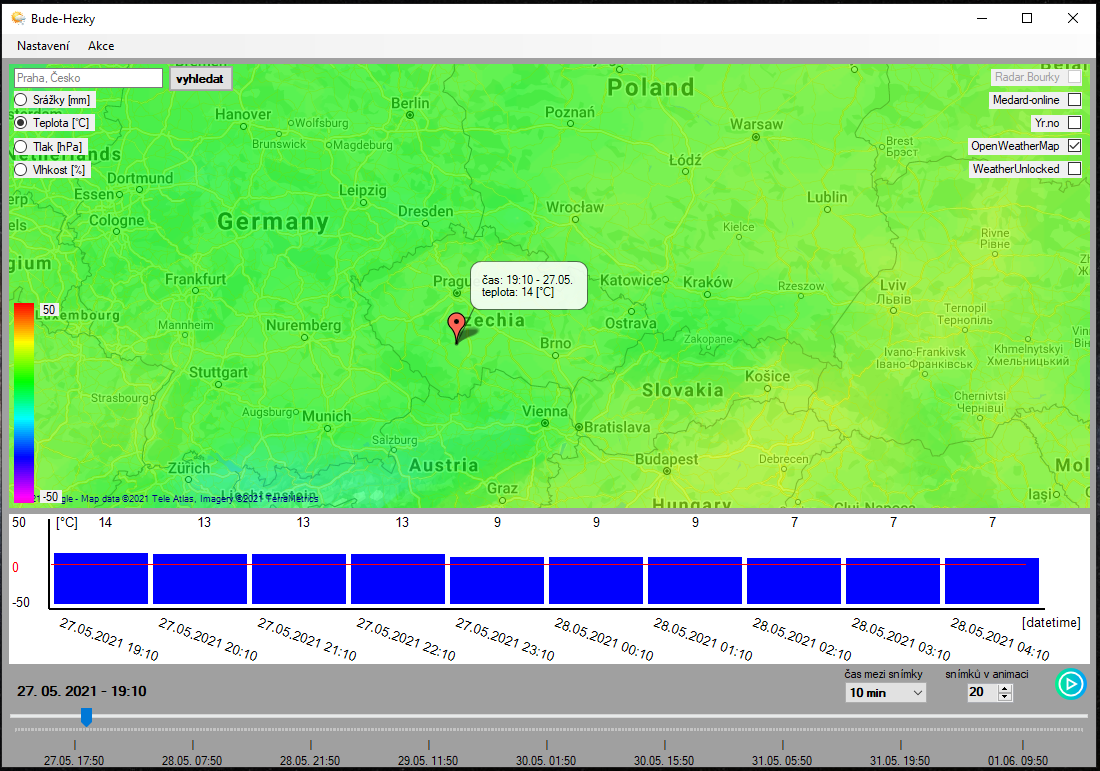
\includegraphics[scale=0.35]{figures/bod počasí.PNG}
			
		\end{figure}
	
	\end{frame}

	\begin{frame}
		\frametitle{Vizualizace dat - Počasí na trase}
		
		\begin{itemize}
			\item Zadání prvku počasí, datových zdrojů, časů a trasy (GPX)
		\end{itemize}
	
		\begin{figure}
			
			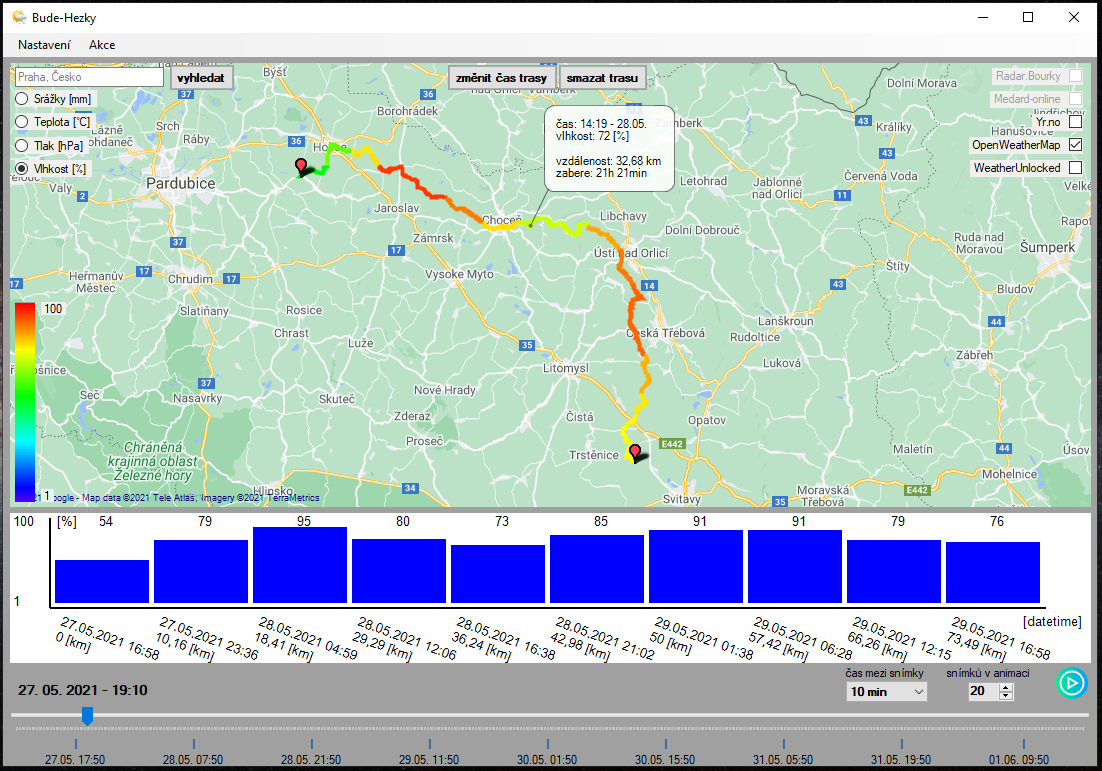
\includegraphics[scale=0.35]{figures/trasa počasí.png}
			
		\end{figure}
		
	\end{frame}

	\begin{frame}
		\frametitle{Závěr}
		
		\begin{itemize}
			\item Různorodost datových zdrojů pro různé účely
			\item Splnění všech požadavků
			\item Možnost rozšíření o nové datové zdroje
			\item Pomalé zpracovávání více datových zdrojů současně
		\end{itemize}
	\end{frame}

	\begin{frame}
		\frametitle{Poděkování}
		
		\begin{center}
			\Huge
			Děkuji za pozornost
		\end{center}
		
	\end{frame}

	\begin{frame}[noframenumbering,allowframebreaks]
		\frametitle{Citace}
		
		\nocite{*}
		
		\printbibliography
		
	\end{frame}
	
\end{document}